\documentclass{article}

\usepackage[utf8]{inputenc}
\usepackage{txfonts}
\usepackage{rotating}
\usepackage{amssymb}
\usepackage{natbib}
\usepackage{varioref}


\begin{document}

%
%  These Macros are taken from the AAS TeX macro package version 4.0.
%  Include this file in your LaTeX source only if you are not using
%  the AAS TeX macro package and need to resolve the macro definitions
%  in the BibTeX entries returned by the ADS abstract service.
%
%  For more information on the AASTeX macro package, please see the URL
%	http://www.ferberts.com/AAS/aastex.html
%  For more information about ADS abstract server, please see the URL
%	http://adswww.harvard.edu/ads_abstracts.html
%

% Abbreviations for journals.  The object here is to provide authors
% with convenient shorthands for the most "popular" (often-cited)
% journals; the author can use these markup tags without being concerned
% about the exact form of the journal abbreviation, or its formatting.
% It is up to the keeper of the macros to make sure the macros expand
% to the proper text.  If macro package writers agree to all use the
% same TeX command name, authors only have to remember one thing, and
% the style file will take care of editorial preferences.  This also
% applies when a single journal decides to revamp its abbreviating
% scheme, as happened with the ApJ (Abt 1991).

\def\aj{\rm{Astronomical Journal}}                   % Astronomical Journal
\def\araa{\rm{ARA\&A}}             % Annual Review of Astron and Astrophys
\def\apj{\rm{Astrophysical Journal}}                 % Astrophysical Journal
\def\apjl{\rm{Astrophysical Journal, Letters}}                % Astrophysical Journal, Letters
\def\apjs{\rm{Astrophysical Journal, Supplement}}               % Astrophysical Journal, Supplement
\def\ao{\rm{Appl.~Opt.}}           % Applied Optics
\def\apss{\rm{Ap\&SS}}             % Astrophysics and Space Science
\def\aap{\rm{Astronomy and Astrophysics}}                % Astronomy and Astrophysics
\def\aapr{\rm{Astronomy and Astrophysics Reviews}}          % Astronomy and Astrophysics Reviews
\def\aaps{\rm{Astronomy and Astrophysics, Supplement}}              % Astronomy and Astrophysics, Supplement
\def\azh{\rm{AZh}}                 % Astronomicheskii Zhurnal
\def\baas{\rm{BAAS}}               % Bulletin of the AAS
\def\jrasc{\rm{JRASC}}             % Journal of the RAS of Canada
\def\memras{\rm{MmRAS}}            % Memoirs of the RAS
\def\mnras{\rm{Monthly Notices of the RAS}}             % Monthly Notices of the RAS
\def\pra{\rm{Phys.~Rev.~A}}        % Physical Review A: General Physics
\def\prb{\rm{Phys.~Rev.~B}}        % Physical Review B: Solid State
\def\prc{\rm{Phys.~Rev.~C}}        % Physical Review C
\def\prd{\rm{Phys.~Rev.~D}}        % Physical Review D
\def\pre{\rm{Phys.~Rev.~E}}        % Physical Review E
\def\prl{\rm{Phys.~Rev.~Lett.}}    % Physical Review Letters
\def\pasp{\rm{Publications of the ASP}}               % Publications of the ASP
\def\pasj{\rm{PASJ}}               % Publications of the ASJ
\def\qjras{\rm{QJRAS}}             % Quarterly Journal of the RAS
\def\skytel{\rm{S\&T}}             % Sky and Telescope
\def\solphys{\rm{Sol.~Phys.}}      % Solar Physics
\def\sovast{\rm{Soviet~Ast.}}      % Soviet Astronomy
\def\ssr{\rm{Space~Sci.~Rev.}}     % Space Science Reviews
\def\rmxaa{\rm{Rev.Mex. de Astronomia y Astrofisica}}    
\def\zap{\rm{ZAp}}                 % Zeitschrift fuer Astrophysik
\def\nat{\rm{Nature}}              % Nature
\def\iaucirc{\rm{IAU~Circ.}}       % IAU Cirulars
\def\aplett{\rm{Astrophys.~Lett.}} % Astrophysics Letters
\def\apspr{\rm{Astrophys.~Space~Phys.~Res.}}
                % Astrophysics Space Physics Research
\def\bain{\rm{Bull.~Astron.~Inst.~Netherlands}} 
                % Bulletin Astronomical Institute of the Netherlands
\def\fcp{\rm{Fund.~Cosmic~Phys.}}  % Fundamental Cosmic Physics
\def\gca{\rm{Geochim.~Cosmochim.~Acta}}   % Geochimica Cosmochimica Acta
\def\grl{\rm{Geophys.~Res.~Lett.}} % Geophysics Research Letters
\def\jcp{\rm{J.~Chem.~Phys.}}      % Journal of Chemical Physics
\def\jgr{\rm{J.~Geophys.~Res.}}    % Journal of Geophysics Research
\def\jqsrt{\rm{J.~Quant.~Spec.~Radiat.~Transf.}}
                % Journal of Quantitiative Spectroscopy and Radiative Trasfer
\def\memsai{\rm{Mem.~Soc.~Astron.~Italiana}}
                % Mem. Societa Astronomica Italiana
\def\nphysa{\rm{Nucl.~Phys.~A}}   % Nuclear Physics A
\def\physrep{\rm{Phys.~Rep.}}   % Physics Reports
\def\physscr{\rm{Phys.~Scr}}   % Physica Scripta
\def\planss{\rm{Planet.~Space~Sci.}}   % Planetary Space Science
\def\procspie{\rm{Proc.~SPIE}}   % Proceedings of the SPIE

\let\astap=\aap
\let\apjlett=\apjl
\let\apjsupp=\apjs
\let\applopt=\ao



%--------------------------------------------------------
\section{Introduction}
\label{sec:introduction}
%--------------------------------------------------------


%--------------------------------------------------------
\section{Model}
\label{sec:model}
%--------------------------------------------------------

We follow the analytic model of a photoevaporated wind described in \citet{1998AJ....116..322H}.
 
The simplest assumpion is that there is a static spherical distribution of gas about the central lowmass star. This gas is being evaporated and ionizing by the radiation coming from $\theta_1 C$

\begin{itemize}
\item{Radiacion ionizante que incide de manera paralela al proplyd.}
\item{Se asume una geometria cilindrica con simetría en la coordenada $\Phi$}
\item{Frontera de ionizacion semiesferica}
\item{El gas fotoionizado fluye de manera radial de la frontera de ionizacion}
\end{itemize}

El flujo no es isotermico
Las desexcitaciones colisionaes no son despreciables

%--------------------------------------------------------
\subsection{Geometry}
\label{sec:geometry}
%--------------------------------------------------------

Si tomamos un marco de referencia cuyo cero se encuentre en el centro
del proplyd, podemos definir una coordenada espacial adimensional $\rm
R = r / r_0$ donde $\rm r_0$ es la distancia medida observacionalmente
del centro del proplyd a la frontera de ionizacion

\begin{figure}[h]
  \centering
  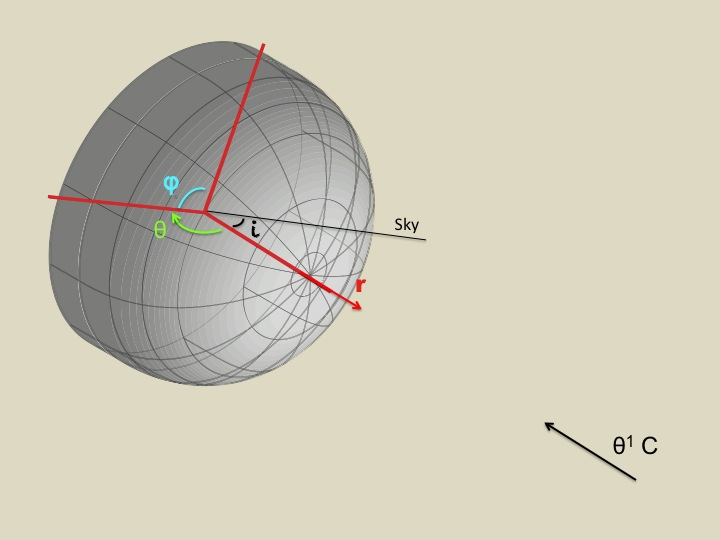
\includegraphics[width=8.5 cm]{./graf_model_3D/geometry_model.jpg}
  \caption{A sketched geometry of the model.} \label{fig:geometry}
\end{figure}

%-------------------------------------------------------
\subsection{Radial Density Structure}
\label{sec:density}
%-------------------------------------------------------

As we mentioned above one way to develope models that take into account both, the radiative transfer and the hydrodinamics of the gas, is to introduce an aproximate hydrodinamics in the radiative models that are availables and such are stables. This is our case and the way to introduce the hydrodinams of the gas is using the electron density structure that is a result of the hydrodinamic teorical models.

We divide the proplyd flow into two zones:

\begin{itemize}
  \item{$\rm r > r_0$: An outer, fully ionized flow.}
    \item{$\rm r < r_0$: An inner, partially ionized flow.}
\end{itemize}

This is equivalent to say that the behavior of the physical conditions are diferent in both zones. We suppose that the flow in the partially ionized zone, that correspond to the thin ionization front, is a subsonic flow. This is acelerated to be a supersonic flow in the outer fully ionized zone. The boundary between them are exactly the sonic point. The conditions there, and in every point of the proplyd, are fixed by continuity, it means that the electron density change as the gas-phase velocity change and visceversa. 

\begin{equation}
  \rm n_e(X) = \left\lbrace
    \begin{array}{l}
      f_1(X) \;\;\;\;\; 1 \ge X \ge 0.98 \\
      f_2(X) \;\;\;\;\;  0.02 \ge X \le 0.98  \\
    \end{array}
  \right.
\end{equation}

%-------------------------------------------------------
\subsubsection{The outer zone}
\label{sec:outer}
%-------------------------------------------------------

In the outer zone we assume an isothermal, supersonic, complite ionized flow. From mass conservation, in spherical geometry and In the steady state, radial velocity of the ionized gas, v(r),
satisfies the equation


\begin{equation}
  \rm \rho v r^2 = cte
\end{equation}

%-------------------------------------------------------
\subsubsection{The boundary}
\label{sec:boundary}
%-------------------------------------------------------

Because the gas velocity is the property that determines the behavior
of other physical properties of the proplyd, the logical boundary
between the regions is exactly the sonic point.

This point is also where the criterion of Stromgren for a density
bounded region is met. That is, where the photoionization balance is
broken and the recombination start to overcome the photoinization.

INSERTAR LA ECUACION

%-------------------------------------------------------
\subsubsection{The inner zone}
\label{sec:inner}
%-------------------------------------------------------

Partially ionized region: Density is function of sound speed

La ley de densidad usada para el gas completamente ionizado como funcion de la velocidad es

\begin{equation}
  \rm R = U^{(-1/2)} exp (\frac{1}{4} (U^2 -1))
\end{equation}

donde $\rm U(R) = v / c_0$ con $\rm v(R)$ la velocidad del gas y $\rm c_0(R)$ la velocidad del sonido.



Y dentro de la frontera de ionización:

\begin{equation}
  \rm \rho(c_m)
\end{equation}

En cada punto la ecuacion de continuidad, permite calcular la densidad:

\begin{equation}
  \rm \rho (R) v(R) R^2 = \rho (R_{max}) v(R_{max}) R_{max}^2
\end{equation}

%--------------------------------------------------------
\section{Results and Predictions}
\label{sec:results}
%--------------------------------------------------------



%--------------------------------------------------------
\subsection{Physical properties}
\label{sec:physical}
%--------------------------------------------------------

\begin{itemize}
  \item{Electron Density: It has an almost constant increase reaching
      the maximum value in the i-front (after the sonic point) where the H is partially
      ionized. In this zone, the electron density reach the critical
      electron density for some ions, making the collisional
      deexitation a process that need to take into account.\\
    This is not important in the outer parts of the flow since they
    are highly ionized, which means that [O III] is the dominant
    coolant. The critical density of this ion is about 1e6 cm-3, which
  is reached just near of the sonic point, that is, where the [O III]
  emission is less than the 10\% of the total [O III] emission. (See
  % Sect.~\ref{\sec:emi}).
}
  \item{Temperature: The electron temperature is almost constant in
      the outer zone. As we approache to the He recombination front
      the Te increase reaching the maximum value just before the
      i-front, where the He is neutral and the H still fully ionized. \\
    It is due for two reasons: The first one is that as the radiation
    field goes into the gas-phase of the proplyd, the less energy
    photons are absorved. This cause a hardening of the radiation
    field increasing the mean electron kinetic energy. That is,
    increasing the photoelectric heating per recombination. The second
  one is the electron density increase. It causes collisional
  deexcitation of the main cooling lines.}
\end{itemize}

%--------------------------------------------------------
\subsection{Ionization structure}
\label{sec:ionization}
%--------------------------------------------------------



%--------------------------------------------------------
\subsection{Emissivities}
\label{sec:emi}
%--------------------------------------------------------

All the high ionization lines are all wholly outside the sonic point.

[Ne II], Ha, [N II] and [O II] have almost the 90\% of their emission
in the supersonic zone and the 10\% in the sub-sonic zone.

[S II] is about 70\% outside the sonic point and 30\% inside.

[O I] is about 20\% outside and 80\% inside the sonic point.

So if we take into account the full emission of the proplyd, and the
sub-sonic zone is not well modelated, the efect of this should be not
very important since it is only going to affect two
lines. Nevertheless, if we want to compare the model predictions with
observations that takes only a little aperture of the proplyd and it
is near of the center (near the i-front), the sub-sonic zone will be
very important.

There are a clear separation of 3 km/s (about 15\%) between the median
velocity of the [O III] 5007 and 4363 lines.

Discutir tambien la diferencia que hay entre la linea auroral y la
nebular de [NII] para ver la importancia de las desexitaciones
colisionales. Una es mas afectada que la otra y por lo tanto conforme
vamos a las zonas de mayor densidad la razon entre ellas debe ir
cambiando, aumentando de hecho.

%--------------------------------------------------------
\section{Conclusion}
\label{sec:conclusions}
%--------------------------------------------------------

We will construct Cloudy models of a series of individual radial cuts from the center of the proplyd, at different angles $\theta$ from the proplyd axis.

\bibliographystyle{t}

\bibliography{model}

\end{document}
